



\chapter{Digital Signal Processing for Nonlinear Phase Noise Compensation}\label{ch:DSP}

After detecting the transmitted signal, the retrieved information is sent to the \textit{digital signal processing} (DSP) module where the signal can be decoded and electronic noise mitigation can be implemented. In this Chapter two DSP schemes that mitigate nonlinear interference noise will be presented. The first method is a electronic compensation technique that has been analytically derived to perform optimal compensation of nonlinear phase shifts~\cite{NLPNDSP,liu2002improving}. This electronic scheme requires the current state of the system (fiber length, number of amplifiers and detected power) to be able to compensate for the acquired phase shift. Having this information is not always possible in a real system. Thus, a second detection scheme is implemented using machine learning to enable a nonparameter detection scheme that can characterize the  nonlinear phase noise as well as other impediments. 


\section{Electronic Compensation of Nonlinear Phase Noise } \label{sec:DSPdig}
As was described in Section~\ref{sec:NLPN} the Gordon-Mollenauer effect induces a nonlinear phase shift to the transmitted signal due to the interaction between the ASE noise and the Kerr effect~\cite{gordon1990phase}. The analytically derived compensation intendeds to add the opposite amount of phase shift to each IQ parameter. Each detected symbol would acquire a phase shift from the DSP scheme proportional to the optimal compensation coefficient $\alpha$~\cite{liu2002improving}. This technique can correct accurately the NLPN acquired due to lumped amplification, but it is very sensitive to perturbation. Thus, if any other NLIN is the dominant noise source in the system, the DSP scheme looses its prediction capabilities and will not be able to accurately compensate the constellation.~\\

\subsection{Optimal Nonlinear Noise Compensation }
Consider the electric field at the detector side after N spans of lumped amplification as $E_{N}=E_{0}+n_{1}+n_{2}+\cdots+n_{N}$, where $E_{0}$ is the transmitted signal and $n_{i}$ is the AWGN of the ith span~\cite{gordon1990phase}. The mean nonlinear phase shift acquired is approximately $\braket{\phi_{NLPN}}=\gamma N L_{eff}P_{N}$ as discussed in previous sections~\cite{NLPNDSP,FiberAgrawal}. In this system the main impairments are the acquired nonlinear phase shift and the AWGN. Thus, the received electric field can be written as  $E_{R}=E_{N}e^{-j\phi_{NLPN}}$ containing both sources of noise~\cite{NLPNDSP}.~\\

To Compensate for the acquired nonlinear phase shift, it is natural to suggest a scheme that rotates the phase as $E_{C}=E_{R}E^{-j\alpha P_{N}}$ where  $P_{N}$ is the output power of the Nth amplifier and $\alpha$ is a \textit{scaling factor}~\cite{liu2002improving}. In Reference~\cite{NLPNDSP} the \textit{optimal scaling factor} is analytically deduced to be 
\begin{equation}
\alpha=-\gamma L_{eff}\frac{N+1}{2}.
\end{equation}
 The implementation of this NLPN compensating technique on a square 16QAM constellation is shown in Figure.~\ref{fig:NLPNvis} with decision regions determined using an \textit{expectation maximization} and \textit{Voronoi diagrams}. Notice from this example that the NLPN phase shift present in Figure~\ref{fig:NLPN16qam} causes misclassification of multiple constellation points. It is also important to observe that an imperfect classification is being performed in Figure~\ref{fig:CHQAM}, suggesting that when to symbols start to overlap not much is there to do generally. ~\\


\begin{figure}[H]
  \centering
   \subfloat[With NLPN]{\label{fig:NLPN16qam}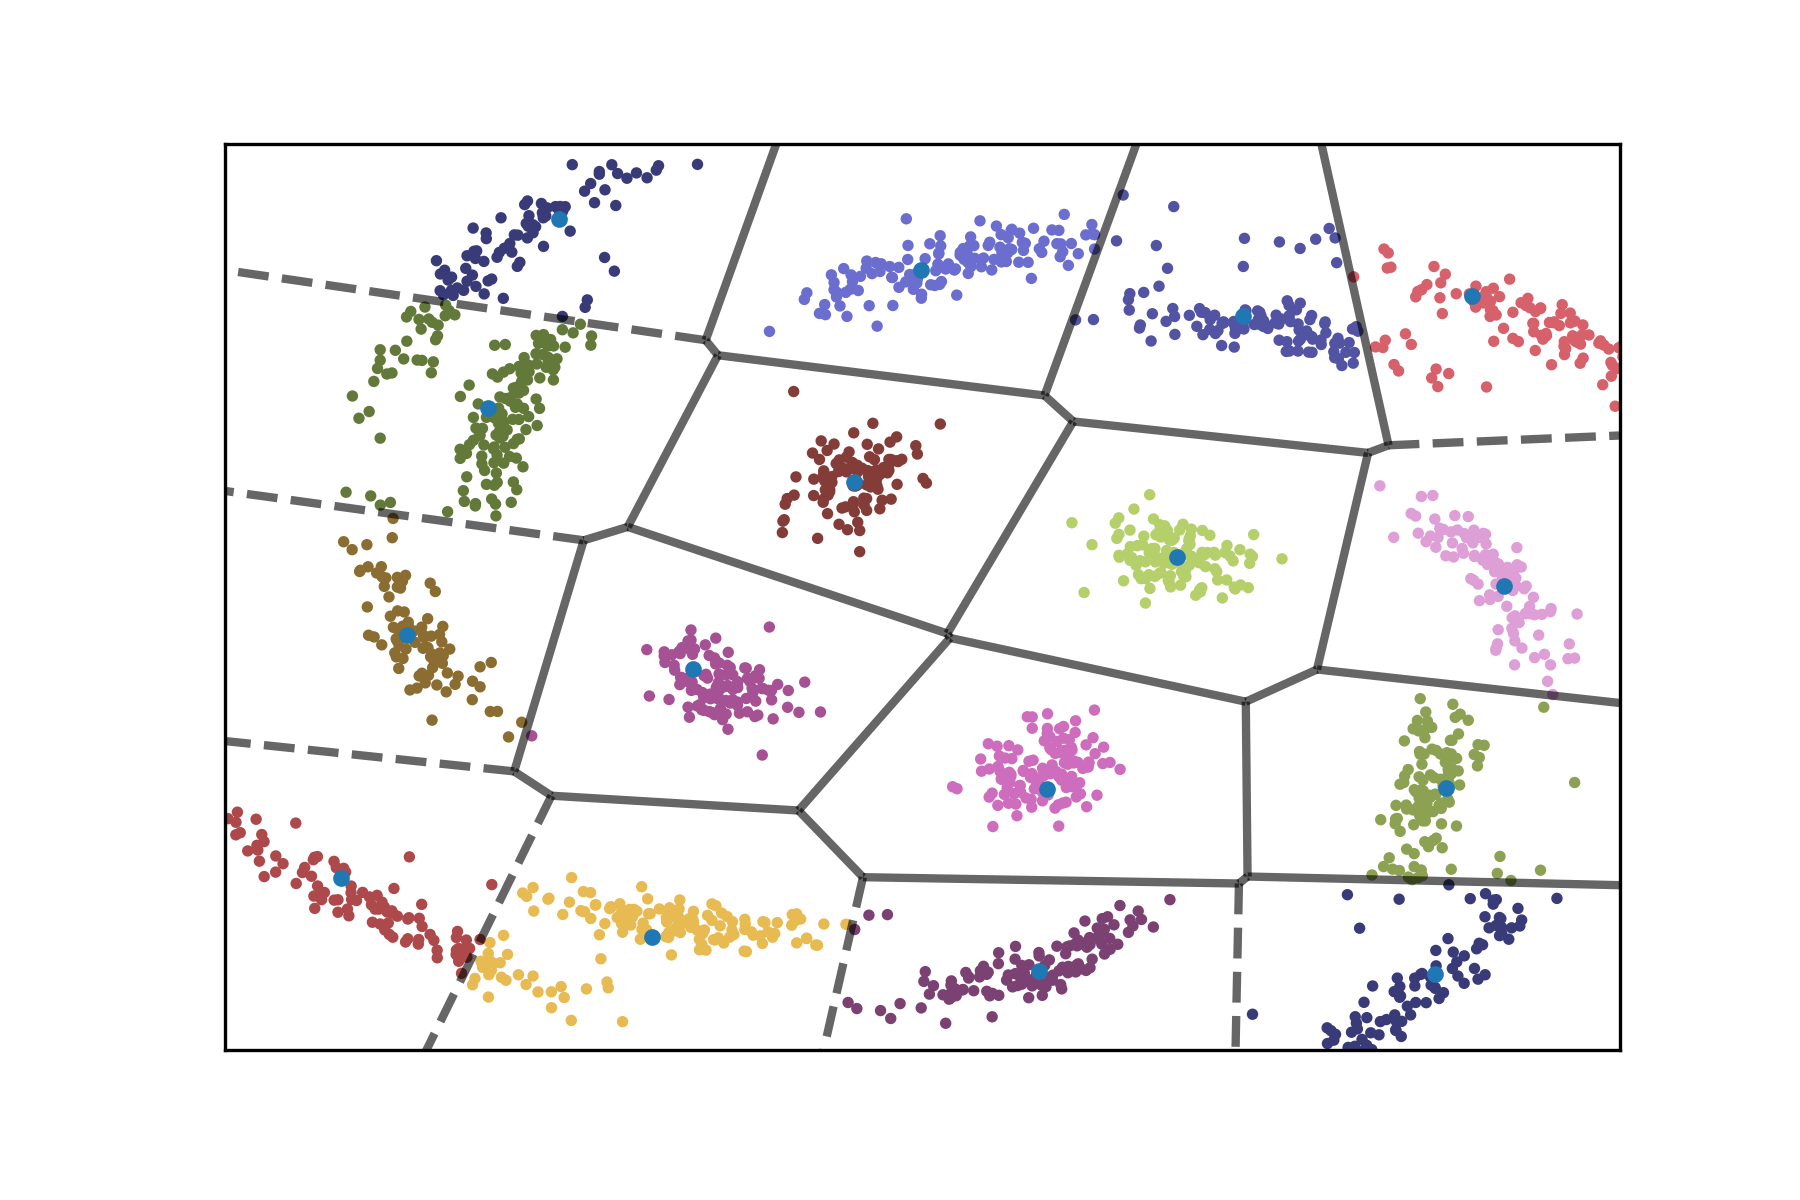
\includegraphics[width=.45\textwidth]{017mw80l40n.png}}
  \qquad
  \subfloat[After NLPN compensation]{\label{fig:CHQAM}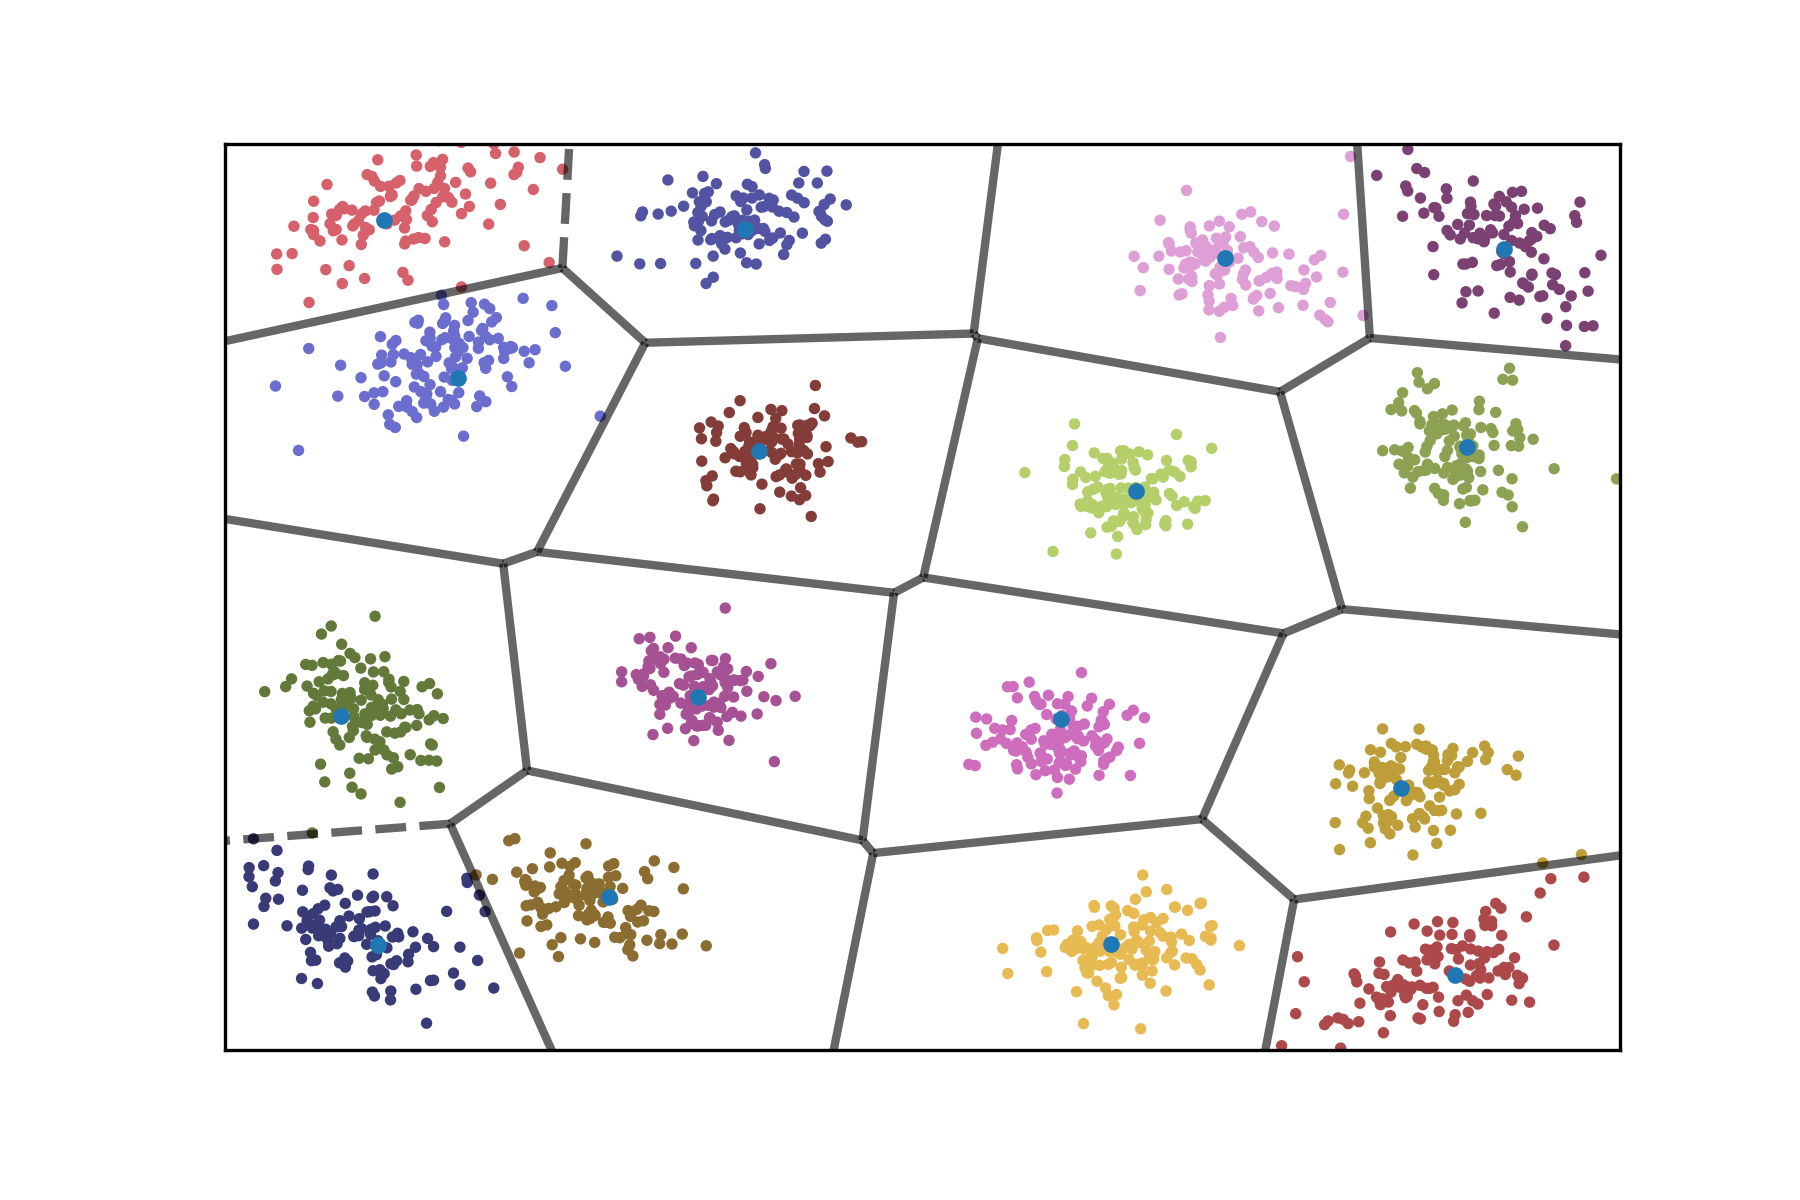
\includegraphics[width=.45\textwidth]{017mw80l40nmit.png}}      
  \caption{Square 16 QAM with a  nonlinear phase shift of $\braket{\phi_{NLPN}}= 0.13$~mrad is shown before and after electronic compensation with optimal scaling factor $\alpha$, as discussed in Reference~\cite{NLPNDSP}.}                                                                                                                                                                                                                                                                                                                                                                                                                                                                                                                                                                                                                                                                                                                                                                                                                                                                                                                                                                                                                                                                                                                                                                                                                                                                                                                                                                                                                                                                                                                                                                                                                                                                                                                                                                                                                                                                                                                                                                                                                                                                                                                                                                                                                                                                                                                                                                                                                                                                                                                                                                                                                                                                                                                                                                                                                                                                                                                                                                                                                                                                                                                                                                                                                                                                                                                                                                                                                                                                         
  \label{fig:NLPNvis}
\end{figure}

As is reported by K. Ho~\cite{NLPNDSP} this compensation scheme can double the transmission distance of a communication system that has as a dominant noise source NLPN. However, it is also acknowledged that other types of nonlinear noise can limit the transmission distance given that only ASE power fluctuations are taken into account. A simple python code can be implemented with this procedure for each detected IQ parameters.

\subsubsection{Implemented Algorithm}

In this section, a short description is given of the compensation scheme implemented in the simulation to compensate NLPN is discussed. This script is executed by a DSP processing module in the simulation software VPI. The function DSP\_ NLPN takes as arguments the IQ parameters detected and request information from the design system through SystemDesign and SystemDesignVolatile. All parameters can be given to the scheme since it has been predefined for the simulation. Each step of the computation is shown in Listing~\ref{lis:NLPN} where the total output of the function gives the compensated IQ components. ~\\
 
\begin{lstlisting}[language=Python, caption= 	Python implementation of a analytically derived compensation scheme to mitigate NLPN. The scheme requires the current state of the system given by user input. ,label=lis:NLPN]
def DSP_NLPN(IQ, SystemDesign, SystemDesignVolatile ):
	# Length of one fiber span [m].
	Lspan = SystemDesign[0]
	# Fiber attenuation [dB/m]
	Att_dB_m = SystemDesign[1]
	# Nonlinear coefficient [1/(W*m)]
	Gamm = SystemDesign[2]
	# Received power W
	Ps = SystemDesignVolatile[0]
	# Number of fiber spans
	NSpans = SystemDesignVolatile[1]
	# Fiber loss
	Att = Att_dB_m/4.343
	# Effective fiber length
	if Att > 0:
		Leff = (1-exp(-Att*Lspan))/Att
	else:
		Leff = Lspan
	# Correction factor
	alpha = -Gamm*Leff*(NSpans+1)/2
	# Perform correction
	IQ_C = IQ*exp(-1j * Ps * alpha)
return IQ_C
\end{lstlisting}

This technique  can correctly compensate NLPN present in one channel. A reference can be drawn to this compensation technique to determine the quality of the mitigation predicted by the ML schemes. The next section will cover the ML algorithms used and the implementation suggested to obtain the best decision regions for a constellation with NLIN. 
\section{Machine Learning Algorithms Implementation  }

The benefit of implementing machine learning to the detection scheme of a communication link is not needing the physical state of the system~\cite{zibar2015application}. This allows the detection scheme to learn about the real impairments of the complete link, computing a accurate decision region for the received constellation. It could be said that training replaces knowledge. This quality makes it a robust system due to the applicability to different systems configurations without the need of making any previous assumptions.~\\

 A drawback of this implementation would be the need to train the scheme when installed or intervened with, requiring a time consuming installation process, if deployed. On the up side, training only has to be done once and it can be performed quickly as well. To initialize the system, a predetermined bit stream would be transmitted as well as being in memory at the receiver side. Since the receiver has the bit stream in memory we get a complete dataset of features and labels. With the dataset a normal training routine can be implemented to any of the algorithms of interest. Given the natures of the dataset, two classification algorithms \textit{support vector machine} (SVM) and \textit{random forest} (RF) will be used to classify a noisy constellation.~\\  


For both of the ML algorithms implemented a simple representation of what training would be can be described as \emph{getting better at a task through practice}. However, uncertainty arises on how to implement an algorithm that exhibits this overall effect. The two principal questions that one encounters are, how does the computer know, if it is getting better, and how does it know how to improve?  Several answers have been proposed, each sprung a class of machine learning in it self. Our task would fall into a class of algorithms categorized under \textit{Supervised Learning}, or algorithms that can learn from exemplars. A training set of examples is given to the algorithm and based on this it generalizes a response for all possible inputs~\cite{marsland2014machine}. A descriptive answer to both of this question will be done for each of the ML algorithms in their corresponding section.




\subsection{Support Vector Machine}




In 1992 V. Vapnik et al. proposed a training algorithm that automatically tunes the capacity of the classification function by maximizing the margin between training examples and class boundary~\cite{boser1992training}. A critical improvement was done to this algorithm when kernels were implemented to solve the nonlinear separable situation~\cite{smola1998learning}. These two techniques are known now as \textit{support vector machine} (SVM), a ML algorithm that transforms a dataset to a higher space and computes a hyper plain that has the maximum margins separating the plane and the data classes~\cite{marsland2014machine}.~\\

\subsubsection{Analytical Description}

 Consider an \textit{input space} of $x(i)$ data points containing two different classes that can not be divided by a linear boundary. Applying a transformation like a projection to higher-dimensional space $v(i)=\varphi(x(i))$ projects the data points into to a space known as a \textit{feature space}, where they could be separated. In this feature space, we can define \textit{hyperplain} as all data points $v(i)$ in $\textbf{v}$ that fulfill $\textbf{w}^{T}\textbf{v}+b=0$, where $\textbf{w}$ is a vector perpendicular to the hyper plane. By defining the support vectors  as all data point $\textbf{v}(i)$ that lay on the hypreplane  $\textbf{w}^{T}\textbf{v}+b=\pm 1$ the maximum margin $b$ can be computed by maximizing $1/||\textbf{w}||$ ~\cite{marsland2014machine,Nonparameter,khan2019optical}. The kernels implemented where a Gaussian radial base function, polynomial combination or a hyperbolic tangent mapping, this transformation are a one to one mapping of the given dataset. A visual description of the algorithm is shown in Figure~\ref{fig:SVMshow} as a general picture we can keep in mind.~\\  
\begin{figure}[h]
\centering
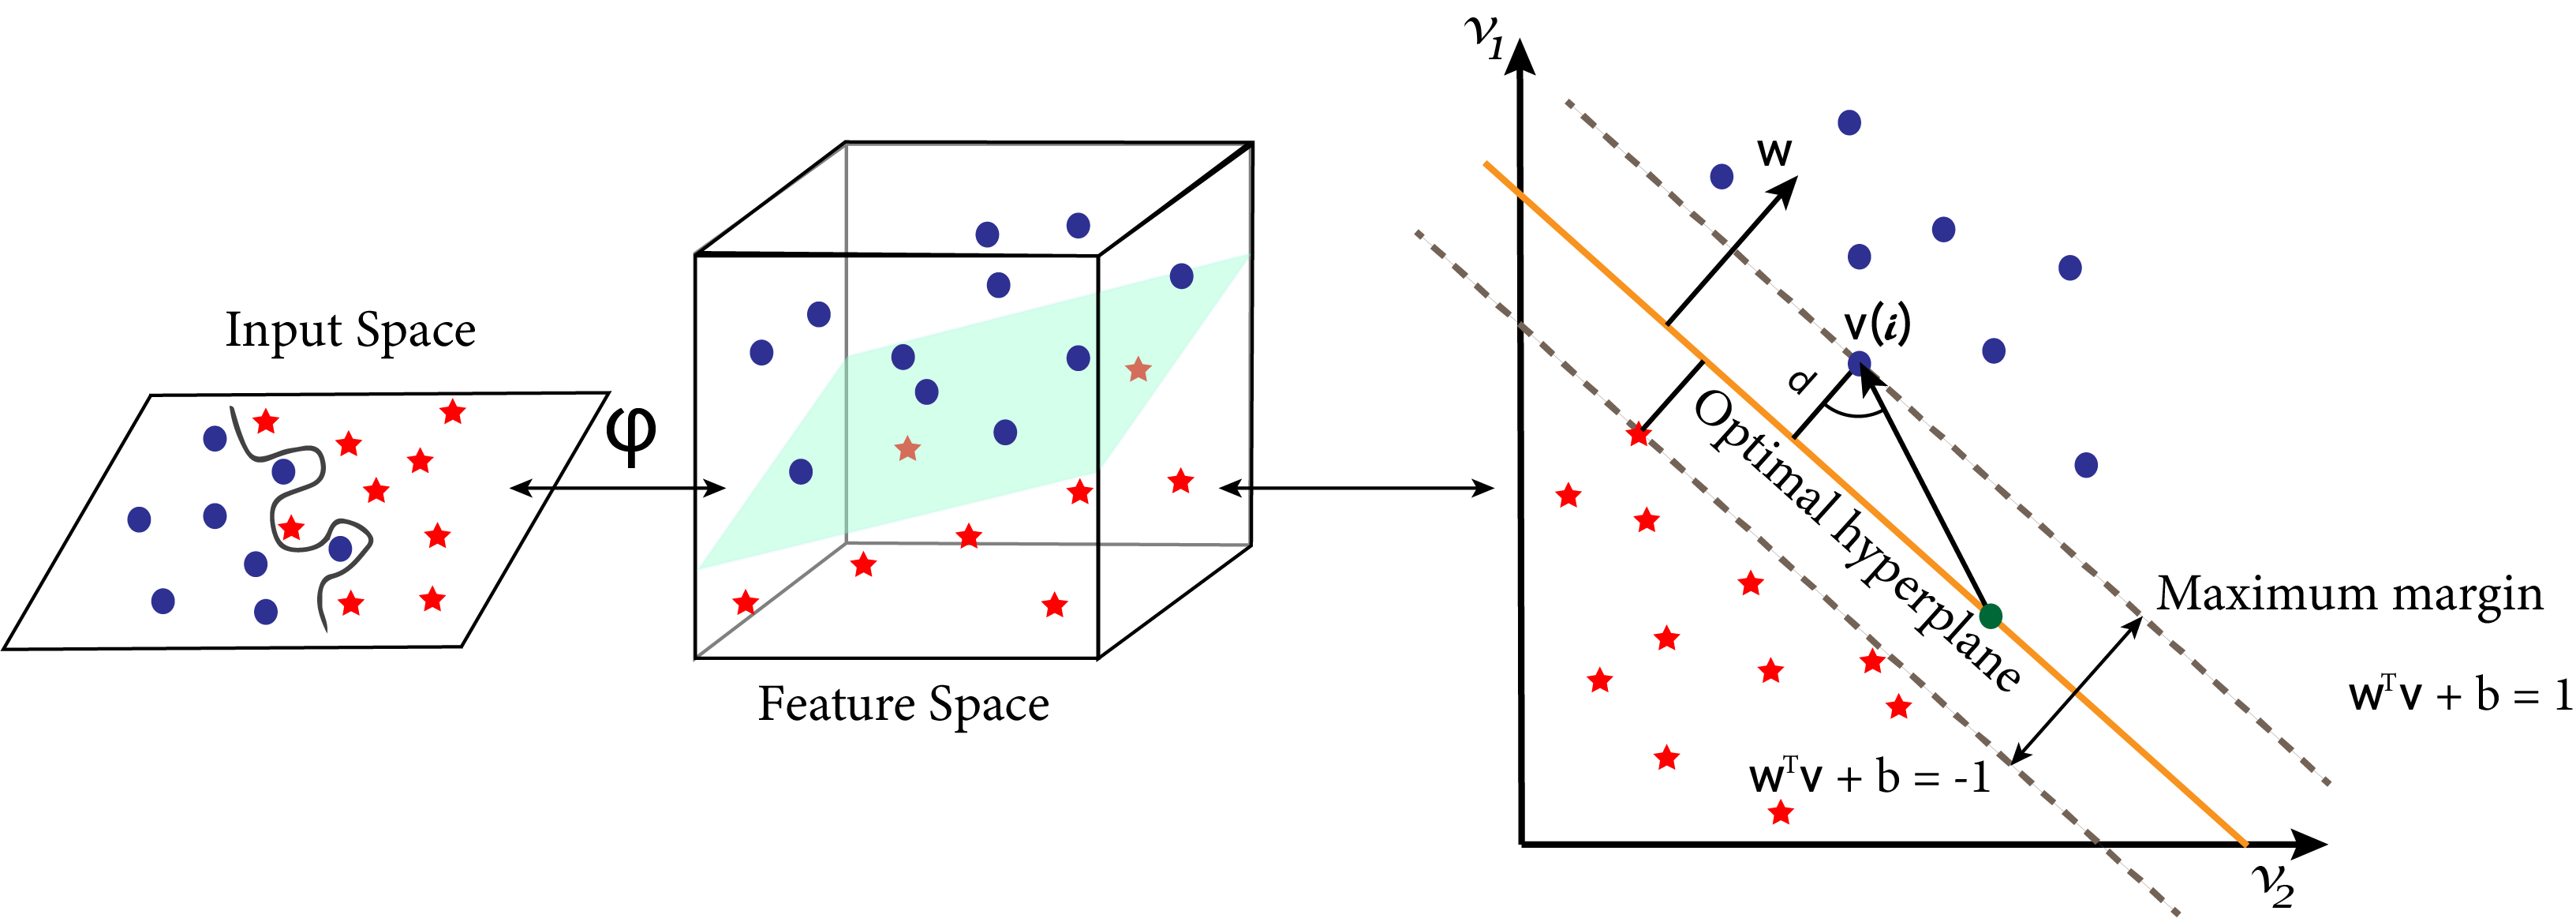
\includegraphics[width=\textwidth]{SVM.png}
\caption{Visualization of the different steps in SVM to find the optimal nonlinear boundary between a dataset with two classes.\\ {\scriptsize Image designed in reference to available figures in Reference~\cite{khan2019optical}}}
\label{fig:SVMshow}
\end{figure}

As a big picture answer the algorithm knows it is getting better if it can decrease the value of $||\textbf{w}||$ subject that all data points are correctly classified. Or written as an optimization problem as
\begin{equation}
\arg\min_{\textbf{w},b}\frac{1}{||\textbf{w}||} \ \ \  \text{   subjec to } y(l)(\textbf{w}^{T}\textbf{v}(l)+b)\geq1 
\end{equation}
where $y(l)$ is a class label given by $\pm 1$ and $\textbf{v}(l)$ is the vector of all data points $v(i)$ with label $y(l)$  ~\cite{boser1992training}. This ML algorithm can be trained to compute nonlinear boundaries dividing data classes in a higher-dimensional space. However, to find the optimal solution one must select the correct transformation (or kernel), the weight of each class and the scaling factor $b$. In the example given a dataset with two classes was described, this was a limitation of SVM in the early 2010. This algorithm  was implemented as NLPN compensation scheme in Reference~\cite{Nonparameter} where a 16QAM constellation is processed by four SVM schemes that detect two classes each, the total response of the classifiers would classify all the sixteen constellation points. These algorithms have been now been optimized and improved such that it is capable of determining multiple classes by an extension of the class label $y(l)$, making it faster to implement and compute. Multiple programming languages can implement this classifier in a few lines of code, in this report Python was used to implement all DSP schemes.
\subsubsection{Implemented Algorithm}

A short description of the python script implemented to compute the optimal parameters for the SVM algorithm is shown in this section. A function DSP\_ SVM returns the optimal parameters (kernel, class weight and scaling factor) for the SVM algorithm given a training dataset. All other functions implemented belong to the \textit{Sklearn} libary in python~\cite{scikit-learn}.

\begin{lstlisting}[language=Python, caption=SVM implementation in python where the optimal parameter are determined form a training dataset. With the optimal parameters the scheme can classify a new set of IQ parameters and determine the decode bit sequence.]
# Computes optimal parameters for SVM given a set of IQ parameters and the decoded bit sequence(BS)
def DSP_SVM(IQ,BS):
	# Split the IQ parameter and BS into test and train sets
    X_train, X_test, y_train, y_test = train_test_split(IQ, BS, test_size = 0.20)
	# Tuning parameters search grid  
	tuned_parameters ={'C': stats.expon(scale=50),
							'gamma': stats.expon(scale=25),
							'kernel': ['linear','rbf', 'polynomial','sigmoid'],
							'class_weight':['balanced', None]}
	# Defines search ledger for SVM  from the different parameter combinations 
    Ledger = RandomizedSearchCV(SVC(), tuned_parameters, cv=4)
	# Computes all combinations given by the ledger and returns the best performing parameters
    Ledger.fit(X_train, y_train)
	# Retrieve optimal parameters with the minimum prediction error 
    Op_param=Ledger.best_params_
    return Op_param
# Compute optimal parameters for the training set of IQ parameters
Op_param = DSP_SVC(IQ_T,BS_T)
# Define the SVM classifier with the optimal parameters
SVMclass = SVC(kernel=Op_param['kernel'],
    					C=Op_param['C'},
    					class_weight=Op_param['class_weight'])
# Train the classifier with the training IQ parameters and BS      
SVMclass.fit(IQ_T,BS_T)
# Predict the BS of the received IQ parameters
BS_R= SVMclass.predict(IQ_R)
\end{lstlisting}
 Notice that two different sets of IQ parameters are implemented in this script. To compute the optimal parameters and define the classifier a set of detected IQ parameters for which we know the decode bit sequences is first used as a training set. Given that the IQ parameters are imprinted with the noise  characteristics of the system and the receiver knows the decode bit sequence this dataset can be used as an input space. After defining and training our SVM classifier it can be implemented to predict on detected symbols transmitted through the same link. 
\subsection{Random Forest}

A \textit{random forest} (RF) or also known as \textit{random decision trees} is a ML algorithm that fits a number of \textit{decision tree classifiers} on different sub-samples of the dataset using averaging over all trees to improve the prediction accuracy and control over-fitting. This algorithm has been developed by incremental incorporation of well understood techniques to optimize its performance and prediction capabilities. By using decision trees, bootstrapping and boosting, three well established techniques, random forest has been developed to be straight-forward to implement and to be trained extremely fast~\cite{ho1995random}. A brief description of the implementation used to characterize NLIN is discussed in this section.
 
   
\subsubsection{Analytical Description}

 Let us first discusses the principal element of this ML algorithm, which is a decision tree. Multiple methods exist to grow a decision tree, the method used in this scheme is known as  \textit{oblique decision trees}~\cite{ho1995random}.  The first step to grow a tree is generating a initial hyperplane that is not necessarily tailored for the dataset of interest. This $d$-dimensional hypreplane can be expressed as $H=(h_{1},h_{2},\cdots,h_{d})$. From this hyperplane the algorithm randomly picks an $h_{i}$ and adds a uniform random variable creating a new hyperplane~\cite{heath1993induction}. For both of this hyperplanes the \textit{sum-minority energy measure} is computed as defined in Reference~\cite{heath1993induction} Theorem 2.1. If the energy difference $\Delta E$ between the two hyperplanes is negative, then the energy of the perturbed hyperplane has decreased and it becomes the current split. If the change in energy increases or stay the same then the perturbed hyperplane has a probability of becoming the new hyperplane or being discarded. To determine when to stop perturbing the current split the energy of all perturbations (around 3000 iterations) is kept to select the split that generated the lowest energy~\cite{heath1993induction}. Although generating this trees can be computed very fast a limiting factor is over-fitting.~\\

\begin{figure}[h]
\centering
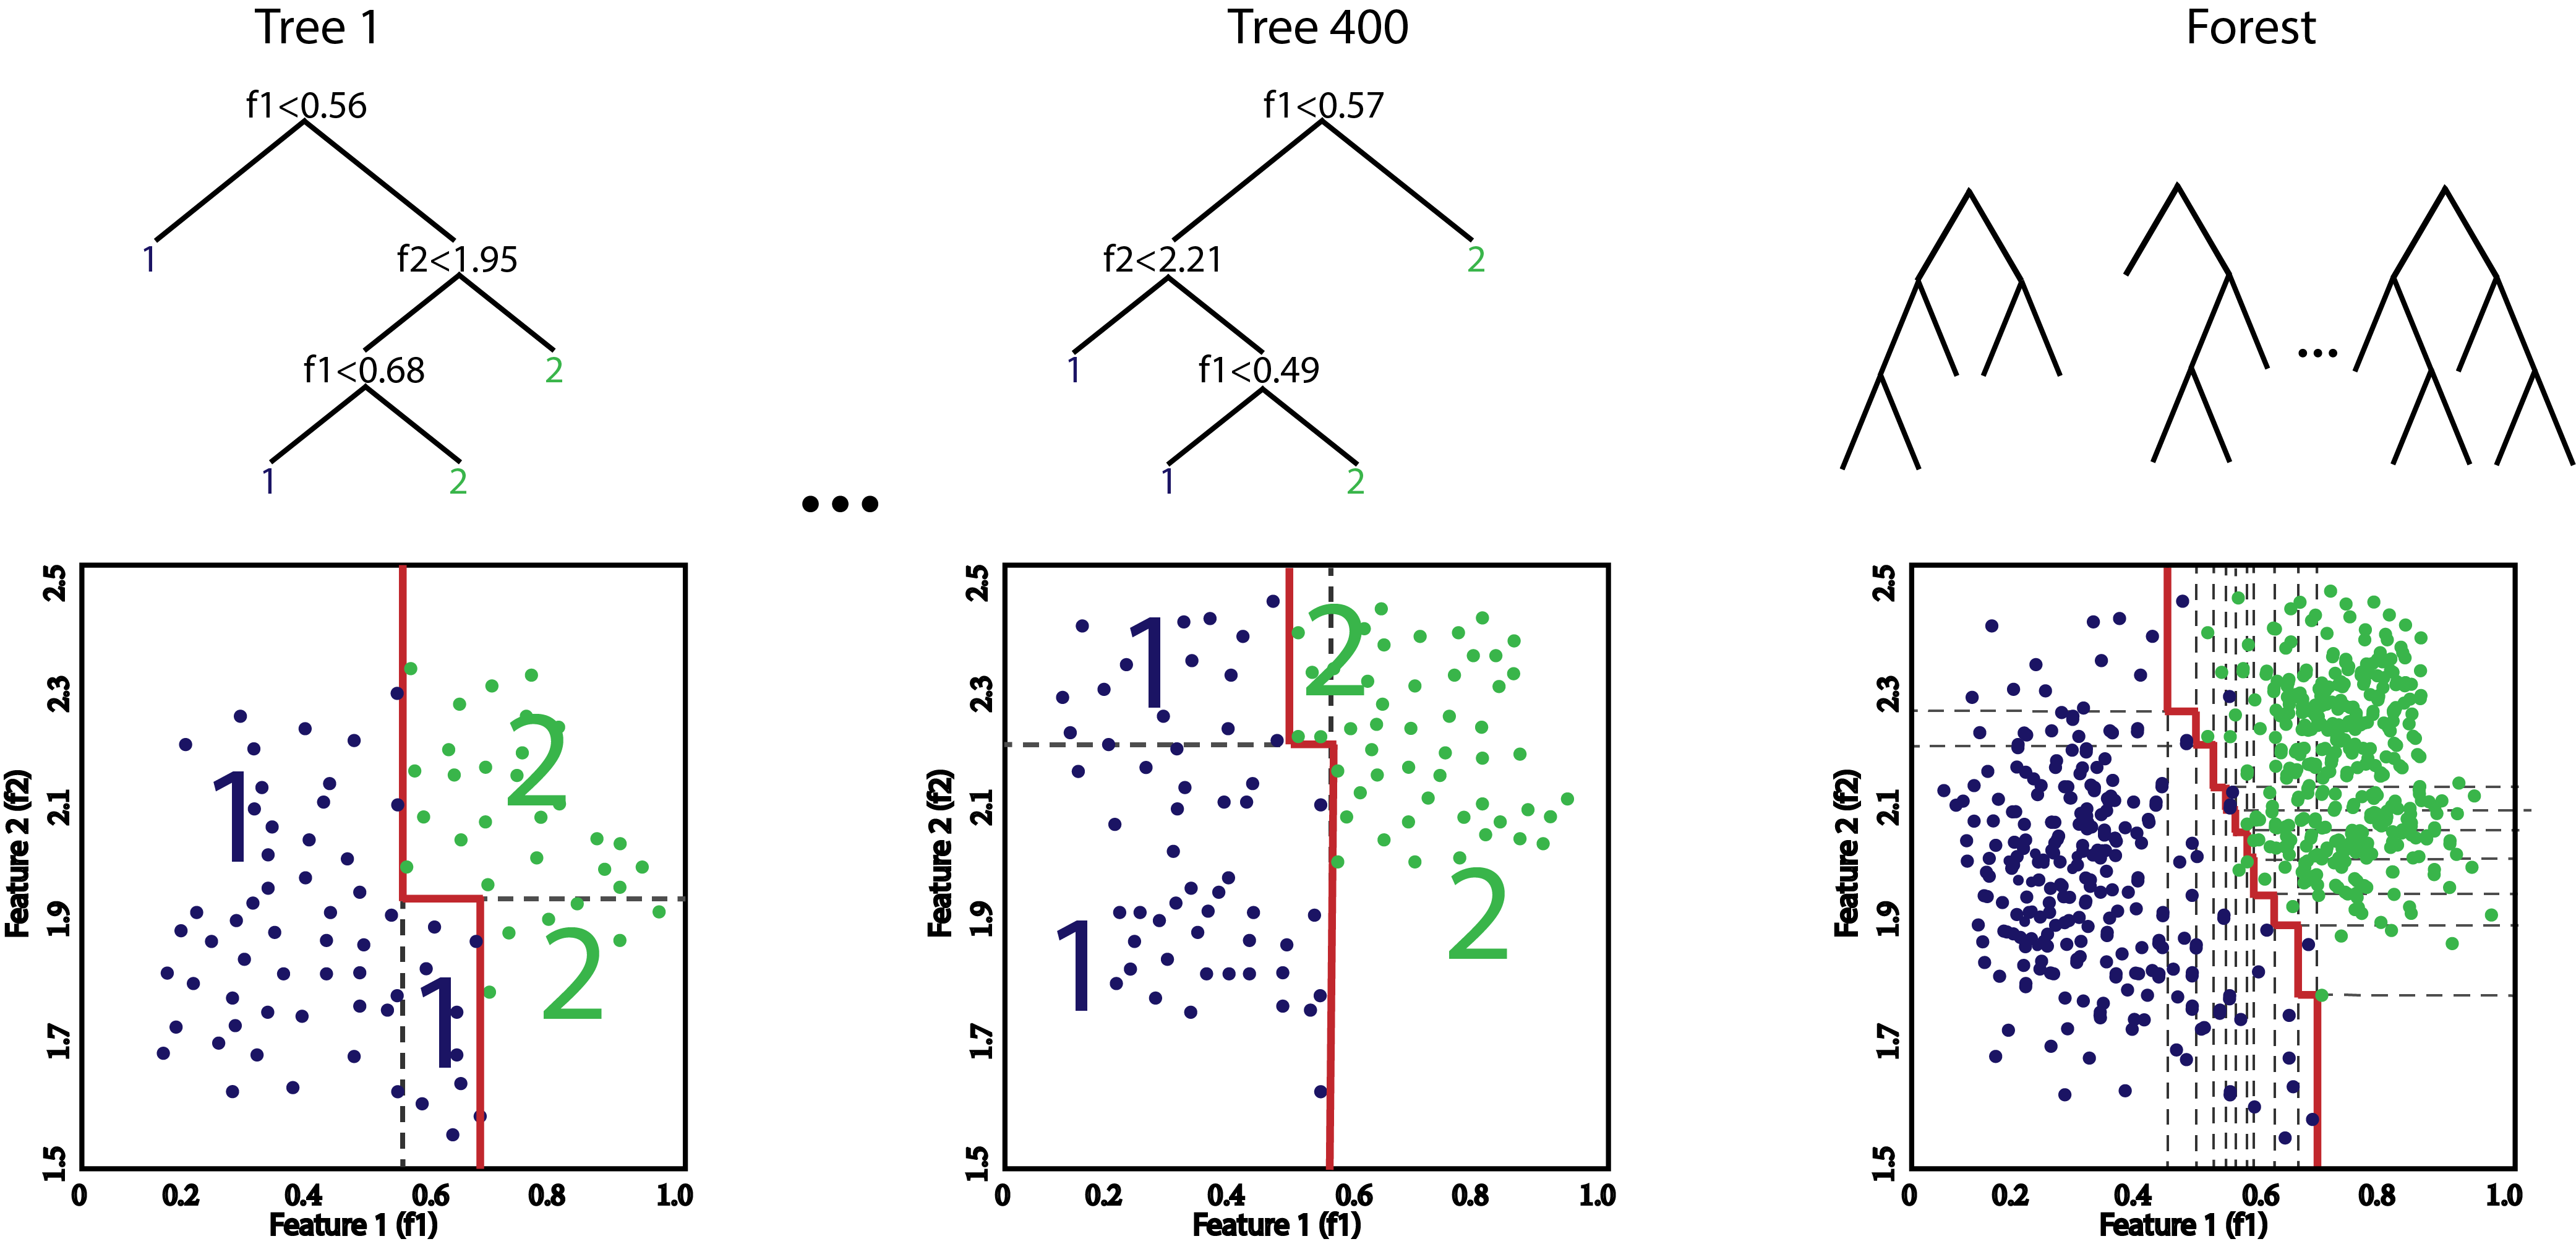
\includegraphics[width=0.9\textwidth]{RandomForest.png}
\caption{ Two different decision trees from a forest are shown  with their computed hyperplane that divides the sub-sampled dataset. When all trees are averaged together a forest is crated giving a decision boundary the is not over-fitted to the original dataset.\\ {\scriptsize Image designed in reference to available figures in Reference~\cite{RFimg}} }
\label{fig:RFshow}
\end{figure}

To counter the effects of over-fitting a dataset, two different techniques are implemented that improve its generalization capabilities. The first technique is \textit{ bootstraping}, which is a sub-sampling dataset technique to increase the training data~\cite{friedman2002stochastic}. Bootstraping creates datasets with the same statistical properties as the original dataset by random sampling with replacement. The second technique is known as \textit{boosting}, where you ensemble a large amount of weak learners to produce a strong learner~\cite{hancock2012bootstrapping}. This three methods compose the basis of a random forest ML algorithm, each of this techniques effect is depicted in Figure~\ref{fig:RFshow}. Implementing random forest can be easily done using multiple programming languages that offer optimized libraries like Python with Sklearn~\cite{scikit-learn}.

\subsubsection{Implemented Algorithm}
Implementing a nonparameter NLIN mitigating algorithm requires training the algorithm in the first instance and then a datasets from the same system can be implemented. Tress are also restrained of growth by delimiting the number of data points (or features), depths of the tree, number of splits and other parameters as shown in Listing~\ref{lis:RF}. The function DSP\_ RandForest takes a set of IQ parameters and its corresponding bit sequence and searches for the optimal parameters to classify this dataset. With the optimal parameters, the algorithm can be trained to obtain the optimal decision boundaries to predict the bit sequence of a detected symbol.    


\begin{lstlisting}[language=Python,caption=Random forest implementation in python where the optimal parameter are determined form a training dataset. With the optimal parameters the scheme can classify a new set of IQ parameters and determine the decode bit sequence.,label=lis:RF]
# Optimal parameters for random forest given a set symbol IQ parameters and the decoded bit sequence BS
def DSP_RandForest(IQ,BS):
# Split the IQ parameter and BS into test and train sets
	X_train, X_test, y_train, y_test = train_test_split(IQ, BS, test_size = 0.2)
# Number of trees in random forest
	n_estimators = [int(x) for x in np.linspace(start = 200, stop = 500, num = 3)]
# Number of features to consider at every split
	max_features = ['auto', 'sqrt']
# Maximum number of levels in tree
	max_depth = [int(x) for x in np.linspace(5, 20, num = 3)]
	max_depth.append(None)
# Minimum number of samples required to split a node
	min_samples_split = [2, 5, 10]
# Minimum number of samples required at each leaf node
	min_samples_leaf = [1,2]
# Create the random grid
	random_grid = {'n_estimators': n_estimators,
               'max_features': max_features,
               'max_depth': max_depth,
               'min_samples_split': min_samples_split,
               'min_samples_leaf': min_samples_leaf}
# Defines search grid of input parameters for the RF 
    Grid = GridSearchCV(RandomForestClassifier(), random_grid, cv = 5)
# perform best parameter search using the train set
    Grid.fit(X_train, y_train)
# Retrieve optimal parameters with the minimum prediction error 
    Op_param=Grid.best_params_
return Op_param
# Compute the optimal parameters
Op_param= DSP_RandForest(IQ_T,BS_T)
# Define the RF structure and tree construction parameters  
	Forest = RandomForestClassifier(max_depth=Op_param['max_depth'],
										max_features=Op_param['max_features'],
										min_samples_leaf=Op_param['min_samples_leaf'],
										min_samples_split=Op_param['min_samples_split'],
										n_estimators=Op_param['n_estimators'])
# Train the RF classifier with the training IQ parameters and BS       
    Forest.fit(IQ_T,BS_T)
# Predict the BS of the received IQ parameters 
    	BS_R=Forest.predict(IQ_R)
\end{lstlisting}



\section{Nonparameter Detection Scheme  }
In the previous sections two different ML algorithms were presented. In this section, both of this algorithms are implemented to obtain a more powerful and reliable algorithm. Random forest can be operational very fast but can present over-fitting which reduces its predictive capability. Support vector machine does not over-fit the training dataset but it requires a longer time to find the optimal parameters and train the algorithm to perform accurate predictions. Both of this algorithms have different advantages and disadvantages, making a joint implementation an interesting idea to balance there short comings.~\\

In this thesis a DSP scheme that computes decision regions that characterize the nonlinear noise present in a 16~QAM coherent optical link is suggested. Our intent for this scheme is improving the amount of correctly classified symbols extending the maximum transmission length. The algorithm computes first  the random forest classifier because of its fast execution time. If the SER of the training dataset is grater than zero then support vector machine is also executed to check if a better SER could be achieved. With both of this ML algorithms the transmission length of the system can be improved for the same transmission link. The structure of the script implemented is shown in Listing~\ref{lis:MLDSP}, the execution time of the complete script can take between 2~s to 45~s to compute the optimal decision regions which is a relatively fast implementation time for the system.~\\								    

\begin{lstlisting}[language=Python,caption=Machine learning enabled DSP scheme that  returns the best performing ML algorithm and its optimal parameter for the training dataset. ,label=lis:MLDSP]
def DSP_ML(IQ_T, BS_T):
# Compute optimal parameters for RF given the training set of IQ parameters
	Op_param_RF = DSP_RandForest(IQ_T,BS_T)
# Define the RF structure and optimal tree construction parameters
	Forest = RandomForestClassifier(max_depth=Op_param['max_depth'],
										max_features=Op_param['max_features'],
										min_samples_leaf=Op_param['min_samples_leaf'],
										min_samples_split=Op_param['min_samples_split'],
										n_estimators=Op_param['n_estimators'])
#	Trains the RF classifier given the training IQ parameters and BS
	Forest.fit(IQ_T,BS_T)
#  Predict the BS using RF for the training IQ parameters
	BS_RF = Forest.predict(IQ_T)
# Check the prediction capacity of the RF classifier 
	if( SER(BS_RF,BS_T )> 0 ):
	# Compute optimal parameters for SVM given the training set of IQ parameters and BS
		Op_param_SVM = DSP_SVM(IQ_T,BS_T)
	# Define the SVM classifier with the optimal parameters 
		SVMclass = SVC(kernel = Op_param['kernel'],
							C=Op_param['C'},
							class_weight=Op_param['class_weight'])
	# Trains the SVM classifier with the training IQ parameters and BS      
		SVMclass.fit(IQ_T,BS_T)
	# Predict the BS using SVM for the received IQ parameters
		BS_SVM = SVMclass.predict(IQ_T)
# If the RF classifier performs no mistake it is returned as the optimal classifier
	else:
   	return 'RF', Op_param_RF
# The prediction capability for both algorithms is compared 
	if(SER(BS_RF,BS_T) > SER(BS_SVM,BS_T)):
	# If SVM performs less mistakes predicting the BS then it is returned as the optimal classifier
		return 'SVM', Op_param_SVM
# If RF performs less mistakes predicting the BS then it is returned as the optimal classifier
	else:
		return 'RF', Op_param_RF
\end{lstlisting}	

To get a better understanding of the difference between the decision regions determined in Figure~\ref{fig:NLPNvis} and the predicted regions computed by the ML algorithm, the RF and SVM predicted regions are shown in Figure~\ref{fig:MLcon}. Notice how RF (Figure~\ref{fig:RFcon}) tends to over-fit the training dataset increasing its SER. However, SVM for the same dataset finds optimal regions that do not over lap, predicting accurately most symbols. From Figure~\ref{fig:MLcon} one can observe the difference on how both algorithms compute the regions by looking at the smoothness of the regions. For this dataset SVM has a lower SER and would  be the optimal DSP scheme.

\begin{figure}[H]
  \centering
   \subfloat[SVM]{\label{fig:SVMcons}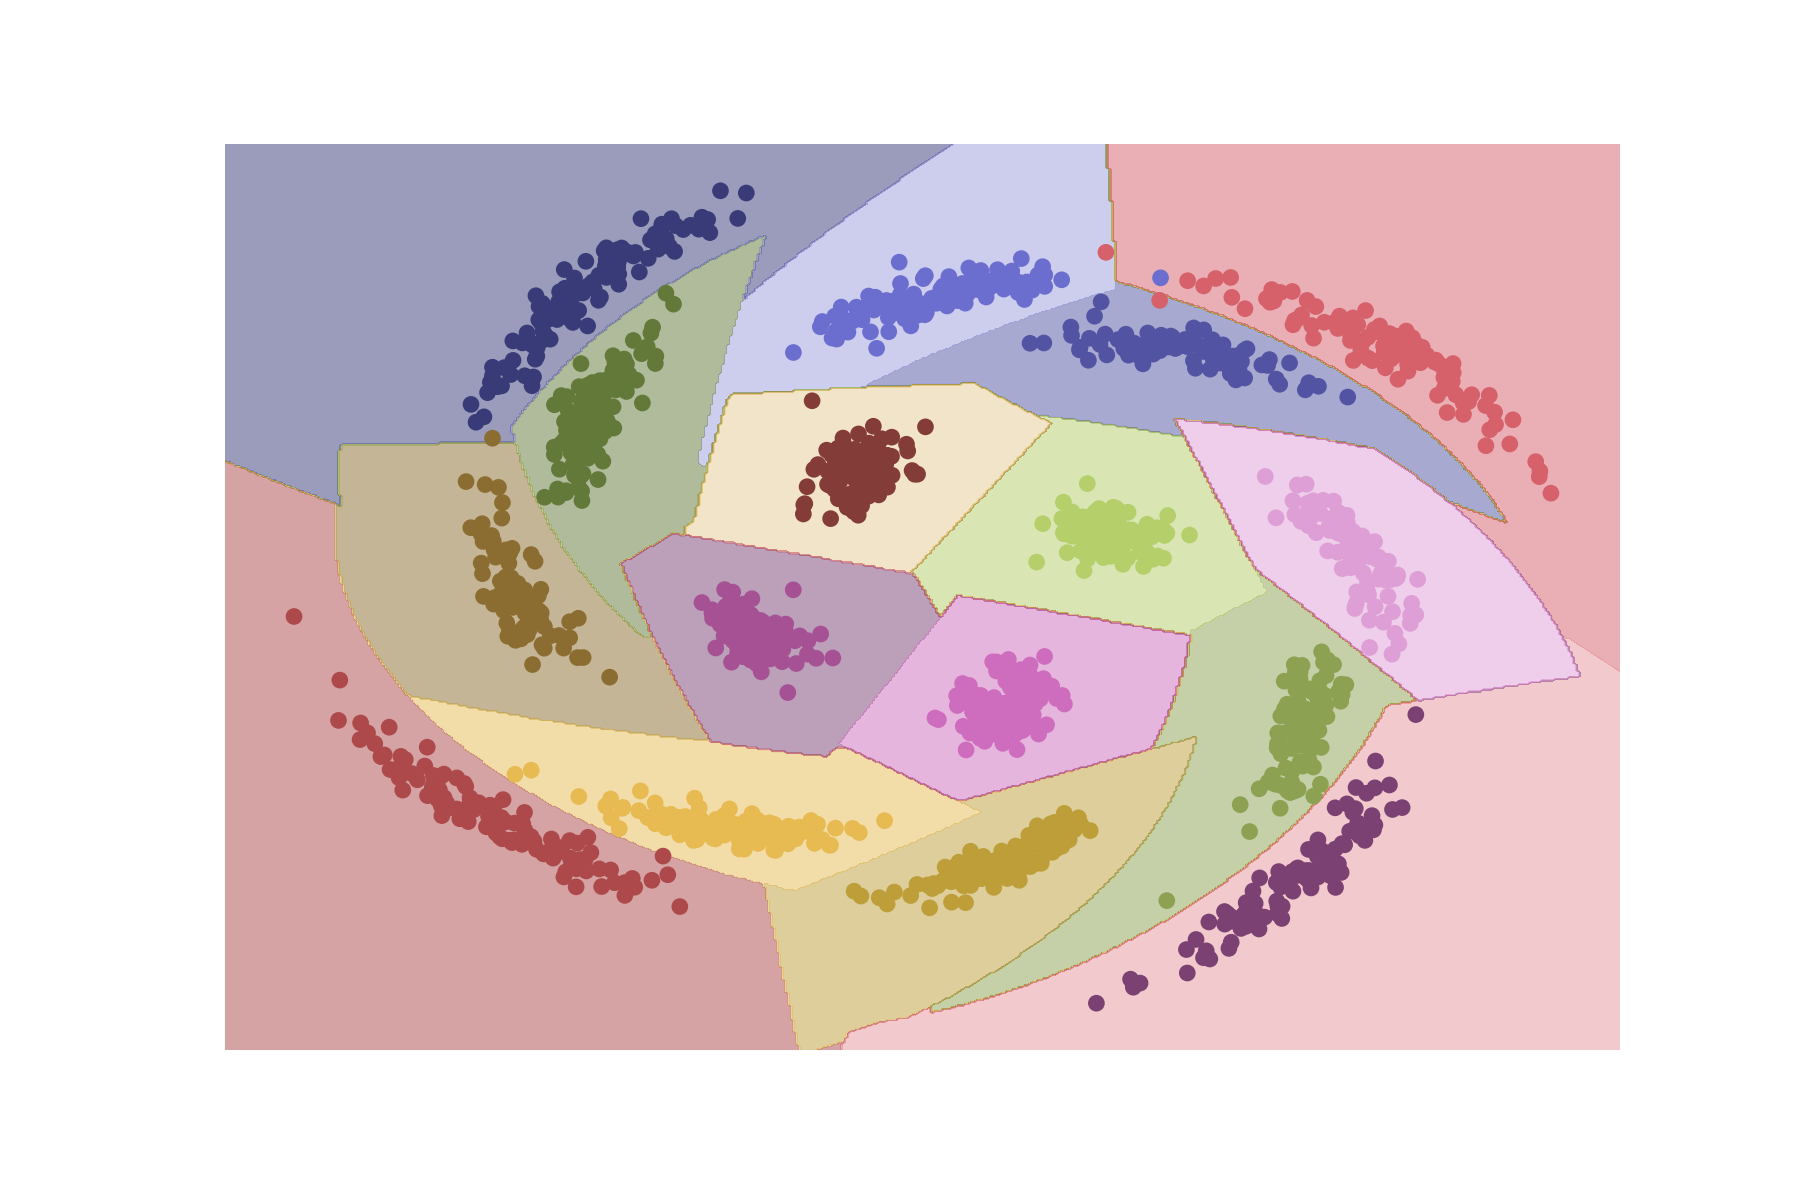
\includegraphics[width=.45\textwidth]{SVCN40L80X.png}}
  \qquad
  \subfloat[Random forest]{\label{fig:RFcon}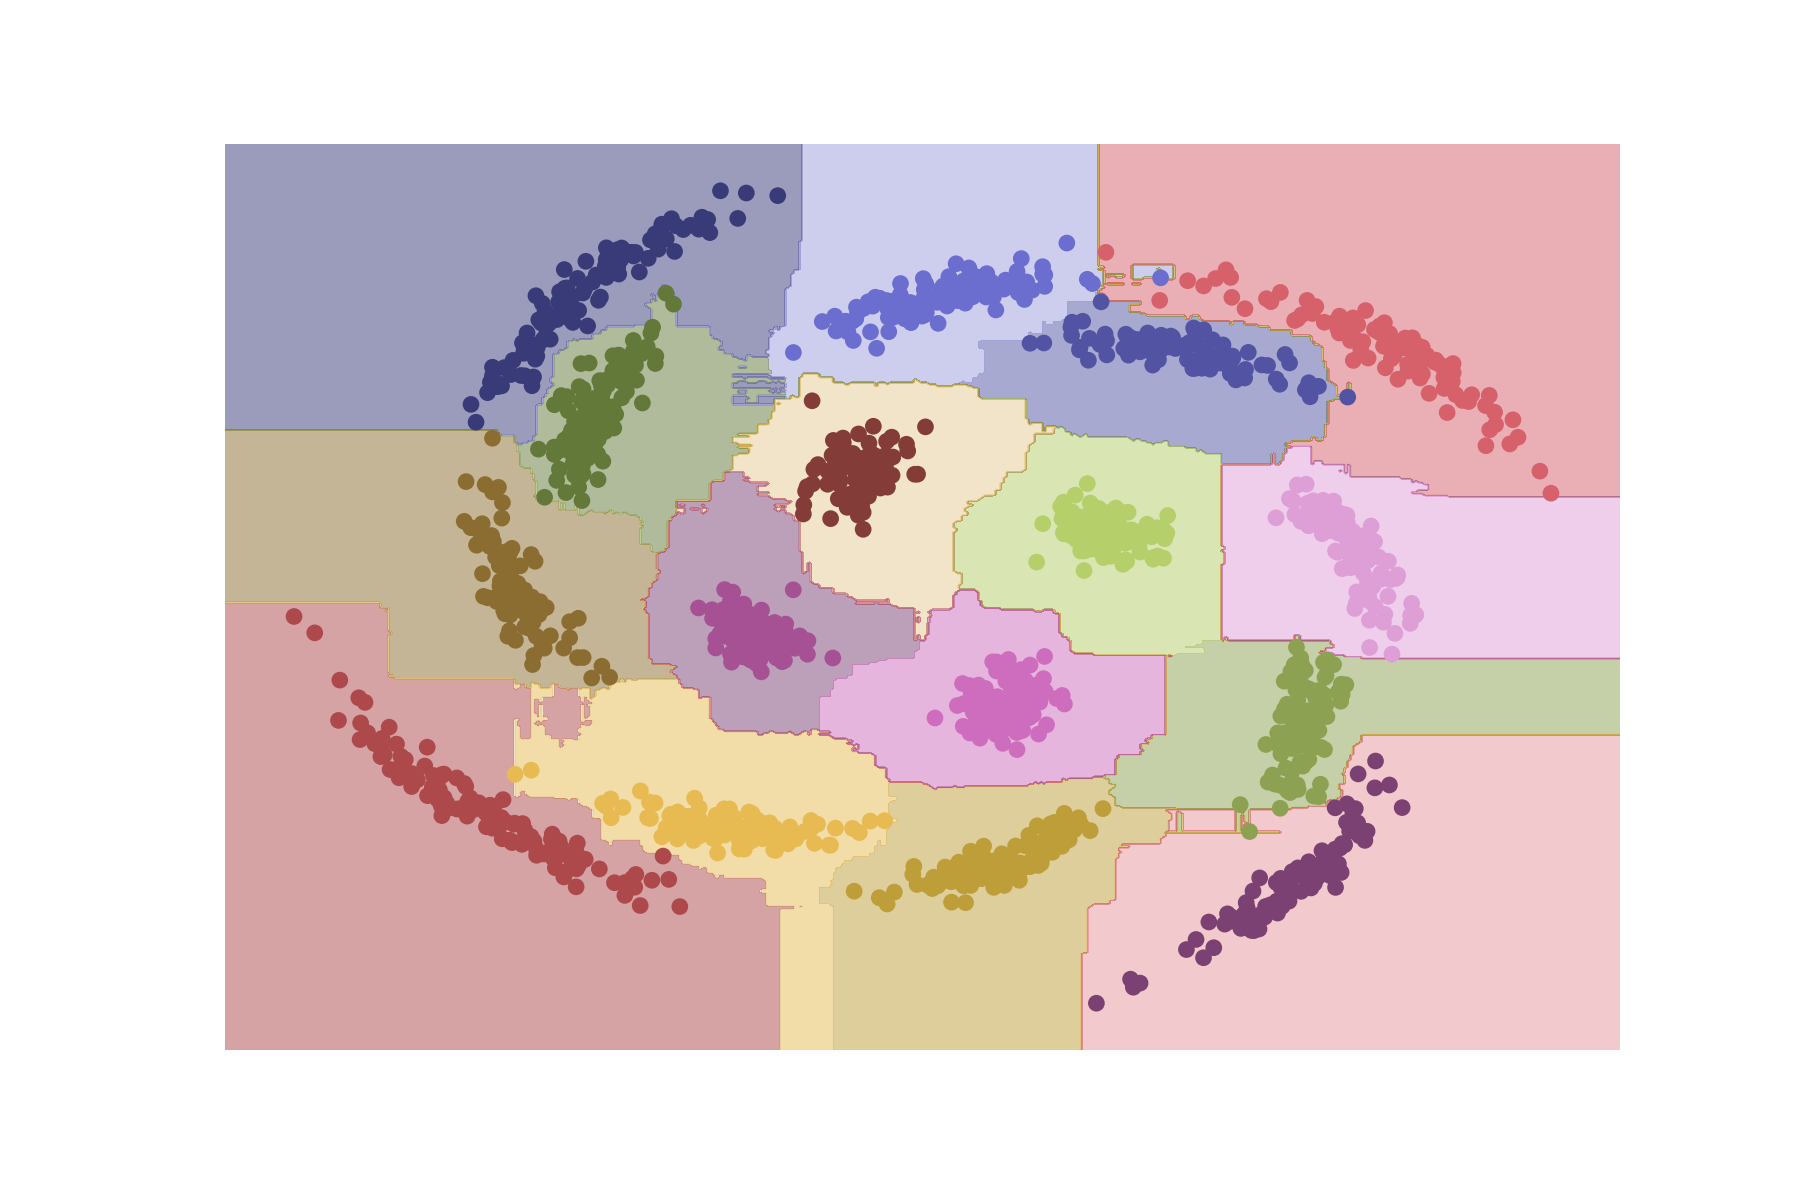
\includegraphics[width=.45\textwidth]{ForeN40L80X.png}}      
  \caption{Square 16 QAM with a nonlinear phase shift of $\braket{\phi_{NLPN}}= 0.13$~mrad is shown. Two different schemes where used to compute the decision boundaries of this constellation, SVM and random forest.}                                                                                                                                                                                                                                                                                                                                                                                                                                                                                                                                                                                                                                                                                                                                                                                                                                                                                                                                                                                                                                                                                                                                                                                                                                                                                                                                                                                                                                                                                                                                                                                                                                                                                                                                                                                                                                                                                                                                                                                                                                                                                                                                                                                                                                                                                                                                                                                                                                                                                                                                                                                                                                                                                                                                                                                                                                                                                                                                                                                                                                                                                                                                                                                                                                                                                                                                                                                                                                                                         
  \label{fig:MLcon}
\end{figure}
Two different communication links were simulated to determine the performance of this DSP scheme. In the next chapter the simulation of the different fiber links will be discussed, as well as the measurements retrieved for the analytical compensation scheme (discussed in Section~\ref{sec:DSPdig}) and the proposed ML algorithm. In the last chapter the conclusions, improvements and further work will be given. 